\chapter{大数相乘}

\section{实验目的}
实现一个大数相乘的程序,输入两个大数,输出它的乘法结果。
\section{实验设计}

% \subsection{GUI设计}
% 本次实验设计的GUI如图所示:
% % \begin{figure}[H]
% %     \centering
% %     \includegraphics[width= 0.9\textwidth]{e:/CourseProject/Assembly/bigNumberMul/assets/2020-06-04-23-43-45.png}
% %     \caption{GUI样式}
% %     \label{GUI样式}
% % \end{figure}


% \subsection{程序流程}
% 创建一个主窗口,之后进入无限消息循环处理模式,当有点击消息产生的时候,根据eax
% 来判断点击的是哪个按钮,并做出相应的动作。

% 比较文件的时候,先打开两个文件,并把他们的句柄保存,之后逐行读取文件并进行比较,
% 最后弹出对话框显示文件的比较结果。

% \subsection{程序流程}
% \begin{enumerate}
%     \item 点击文件1选择按钮,弹出文件选择对话框
%     \item 选择文件1,记录文件1路径
%     \item 点击文件2选择按钮,弹出文件选择对话框
%     \item 选择文件2,记录文件2路径
%     \item 点击比较按钮
%     \item 分别从两个文件中读取两行
%           \iitem 如果两行长度均为0,跳转至7
%           \iitem 若有一行长度不为0,则进行比较,比较完成后跳转至6
%     \item 将结果数组中的数字转化为字符串
%     \item 弹出包含有比较结果的窗口
% \end{enumerate}
\subsection{程序流程}
\begin{enumerate}
    \item 输入两个字符串;
    \item 计算输入字符串的长度;
    \item 逆序存放数据到数组中;
    \item 进行大数相乘;
    \item 对数组中的每一项进行进位处理;
    \item 逆序输出结果。
\end{enumerate}

\section{具体实现}
该节介绍了代码中的部分核心算法和具体代码,包括了计算字符串的长度、逆序存放、数组相乘、进位处理、逆序输出。

\subsection{计算字符串长度}
流程如下:
\begin{enumerate}
    \item 取出字符串的地址;
    \item 取出字符串地址的长度;
    \item 循环取出字符串;
    \item 判断是否为0;
        \iitem 如果为0,则跳出循环;
        \iitem 否则,继续;
    \item 字符串的地址加1,长度加1。
\end{enumerate}

具体代码如下:
\begin{lstlisting}
;计算输入字符串的长度
;stdcall可以自动平衡堆栈
getLen proc stdcall	numstring:ptr byte,numLen:ptr DWORD	
    ;ecx清0,便于循环计数	
    xor ecx,ecx		
    ;esi保存numstring的首地址											
    mov esi,numstring	
    ;edi保存numLen的地址										
    mov edi,numLen												
L1:
    mov al,[esi]
    cmp al,0
    jz  L2
    inc ecx
    inc esi
    jmp L1
L2:
    mov [edi],ecx
    ret   
getLen endp

\end{lstlisting}

\subsection{逆序存放到数组}
逆序存放到数组中,方便在计算乘法后进位不用考虑溢出。

流程如下:
\begin{enumerate}
   \item 取出字符串地址;
   \item 取出相应数组的地址;
   \item 给计数器ecx赋值长度,便于循环;
   \item 取出字符;
   \item 判断是否为负号;
    \iitem 如果是负号,给标记negNum加1,由于负号是第一个字符,也跳出循环;
    \iitem 否则,给字符-“0”得到对应字符的数值;
  \item 直到计数器为0,跳出循环。
\end{enumerate}

具体代码如下:
\begin{lstlisting}
;将得到的字符串转化为数字逆序保存在数组中
revNum	proc stdcall	
    numString:ptr byte,numArray:ptr DWORD,numLen:ptr DWORD
    mov esi,numArray
    mov edi,numLen
    mov ecx,[edi]
    mov edi,numString
    xor eax,eax
L1:
    mov al,[edi][ecx-1]
    cmp al,45
    jz  L2
    sub eax,30H
    mov [esi],eax
    add esi,4
    loop L1
    ret
L2:
    add negNum,1	;此时肯定是最后一个字符串
    mov edi,numLen
    mov eax,[edi]
    dec eax
    mov [edi],eax
    ret 
    
revNum endp	
\begin{lstlisting}
    
\end{lstlisting}

\subsection{数字相乘}
将得到数组中的每一个元素对应相乘再相加

流程如下:
\begin{enumerate}
   \item 先进行外层循环(计数器为esi),如果循环次数大于num1的长度,结束函数;
   \item 进行内层循环(计数器为edi),对edi清0,取num1[esi]分别与num2[edi]相乘,相加到对应的num3[esi+edi]即可;(注意这里的esi和edi不考虑地址,代表数组的第几个数)
\end{enumerate}


具体代码如下:
\begin{lstlisting}
;进行大数相乘(两层循环)
numMul	proc	stdcall 
        num1:ptr dword,num2:ptr dword,num3:ptr dword,
        len1:dword,len2:dword,len3:ptr dword

    ;第一层循环的计数
    xor esi,esi	
    ;第二层循环的计数									
    xor edi,edi										
    mov edx,num1
    mov ebx,num2
    mov ecx,num3
    
L2:		
    ;第一层循环	
    xor edi,edi
    cmp esi,len1
    ;小于len1
    jb L3	
    mov eax,len1
    add eax,len2
    sub eax,1
    mov esi,len3
    mov [esi],eax
    ret
L3:		
    ;第二层循环											
    mov edx,num1
    mov eax,[edx+esi*4]
    cmp edi,len2
    jnb L1
    ;结果保存在EDX:EAX
    mul DWORD PTR [ebx+edi*4]
    add [ecx+edi*4],eax
    sub edi,esi
    inc edi
    jmp L3
L1:
    inc esi
    jmp L2

numMul endp

\end{lstlisting}

\subsection{进位处理}
对num3数组中的每一个数判断是否大于10,大于10,则/10向前进位,修正当前数值为\%10的结果。

流程如下:
\begin{enumerate}
    \item 取出每一个元素值;
    \item 判断是否大于10;
        \iitem 大于10,则修正当前元素值为\%10的结果,往前进位相应/10的结果;
        \iitem 否则,继续执行;
    \item 对最后一个值的时候要单独判断一下,如果往前进了位,那么num3的长度要相应加1。
\end{enumerate}

具体代码如下:
\begin{lstlisting}
    ;进位处理
    carry	proc	stdcall
    	numArray:ptr DWORD,numLen:ptr DWORD
        mov esi,numArray
        mov edi,numLen
        xor ecx,ecx
        
    L1:
        cmp ecx,[edi]
        jnb	L2
        mov eax,[esi+ecx*4]
        mov ebx,0AH
        xor edx,edx
        div ebx
        cmp eax,0
        jnz L3
        inc ecx
        jmp L1
    L2:	
        mov eax,[esi+ecx*4]
        cmp eax,0
        jnz	L4
        ret
    L3:
        mov [esi+ecx*4],edx
        inc ecx
        add [esi+ecx*4],eax
        jmp L1
    L4:
        mov eax,[edi]
        add eax,1
        mov [edi],eax
        ret
    
    carry endp
\end{lstlisting}

\subsection{逆序输出}
对每一个数组逆序输出,这里要注意是否有负号

具体代码如下:
\begin{lstlisting}
    printArray	proc	stdcall	numArray:ptr DWORD,numLen:DWORD
	mov ecx,numLen
	mov esi,numArray
	cmp negNum,1
	jz L3
L1:
	mov eax,[esi][ecx*4-4]
	pusha		;调用C函数要保存寄存器现场
	invoke printf, offset szNumprint,eax
	popa
	loop L1
	ret
L3:
	pusha
	invoke printf,offset szNegSign
	popa
	jmp L1

printArray endp

\end{lstlisting}
\section{实验结果展示}

\subsection{输入正数}
\begin{figure}[H]
    \centering
    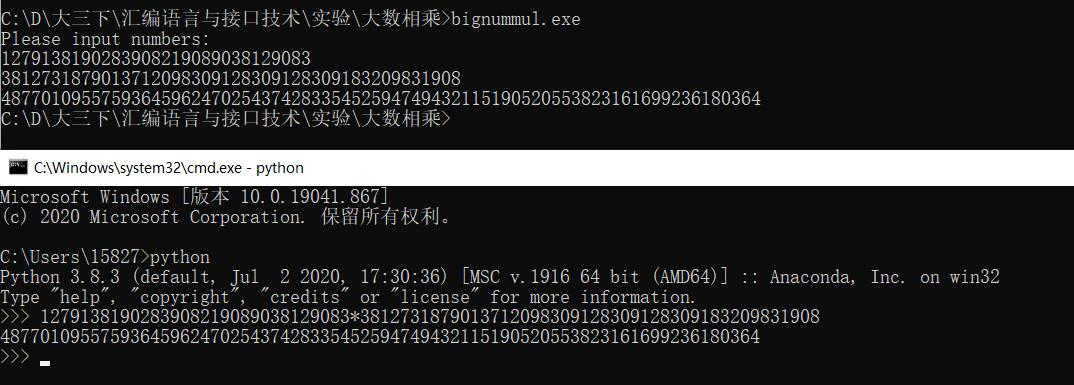
\includegraphics[width= 0.9\textwidth]{assets/大数乘法1}
    \caption{验证1}
    \label{验证1}
\end{figure}
\subsection{输入负数}
\begin{figure}[H]
    \centering
    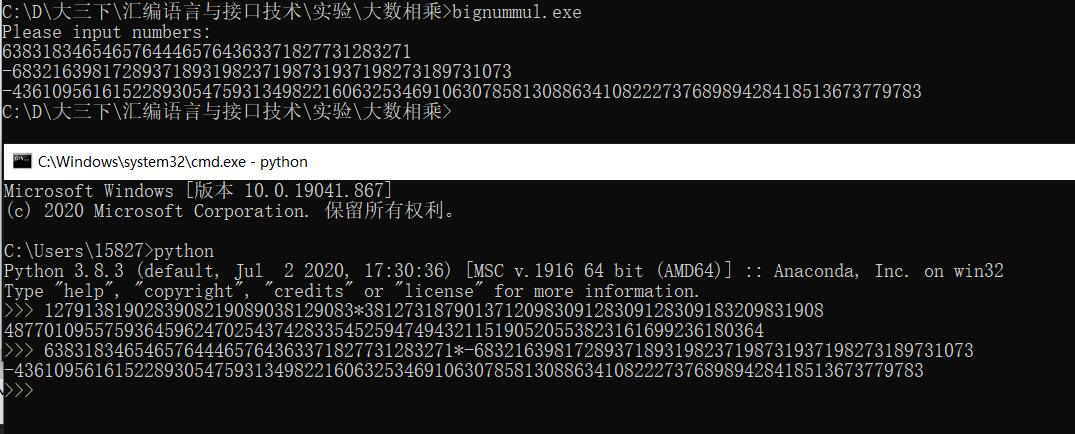
\includegraphics[width= 0.9\textwidth]{assets/大数乘法2}
    \caption{验证2}
    \label{验证2}
\end{figure}

